\documentclass[a4paper]{article}

\usepackage{ReportTemplate}

\usepackage{setspace}
\usepackage{amsmath}
\usepackage[hidelinks]{hyperref}
\usepackage{algorithm}
\usepackage{algorithmicx}
\usepackage{algpseudocode}
\usepackage{subcaption}

\linespread{1.25}

\raggedbottom
\title{SVM的实现以及核函数探究}
\name{涂宇清}
\studentid{522030910152}

\begin{document}

\pagenumbering{arabic}
\pagestyle{headings}

\maketitle

% \section{LaTeX写作示例}

% 本章提供使用LaTeX书写报告时可能使用的各种文档对象的使用示例。\textbf{请在报告写作完成后删
% 除本章。}

% \subsection{公式}

% 示例如式\ref{eq:公式引用名}。

% \begin{equation}
%   \pi = \dfrac{3.1415926}{1}
%   \label{eq:公式引用名}
% \end{equation}

% \subsection{图像}

% 示例如图\ref{fig:图片引用名}。

% \begin{figure}[htb]
%   \centering
%   \includegraphics[scale=0.7]{figs/voice.png}
%   \caption{图片标题}
%   \label{fig:图片引用名}
% \end{figure}

% \subsection{表格}

% 示例如表\ref{tab:表引用名}。

% \begin{table}[th]
%   \caption{表标题}
%   \label{tab:表引用名}
%   \centering
%   \begin{tabular}{ l c r }
%     \toprule
%     \textbf{左对齐} & \textbf{居中对齐} & \textbf{右对齐} \\
%     \midrule
%     内容 & 内容 & 内容 \\
%     内容 & 内容 & 内容 \\
%     \bottomrule
%   \end{tabular}
% \end{table}

% \subsection{代码}

% 示例如下。

% \begin{lstlisting}[language=python]
% # 这是注释
% def func(a, b):
%     print("Hello, world!")
% \end{lstlisting}

\section{简介}
支持向量机(SVM)是一种常用的分类算法,其基本思想是找到一个最优的超平面,使得数据点到超平面的距离最大化,从而实现对数据的分类。

在本次大作业中,我们将不使用现有的机器学习库函数,从零开始实现SVM算法,探究不同核函数、多个核函数组合对SVM算法的影响,并在MNIST数据集和CIFAR-10数据集上进行测试。

\section{算法描述}
\subsection{支持向量机}
对于两类数据,如果其线性可分,那么存在一个超平面$w^Tx+b=0$,使得对于任意数据点$x_i$,若$w^Tx_i+b>0$,则$x_i$属于第一类;若$w^Tx_i+b<0$,则$x_i$属于第二类。而我们需要找到一个最优的超平面,即数据点中到超平面的最小距离最大。这些距离超平面最近的点就是支持向量。

由数据点到超平面的距离公式可知,对于任意数据点$x_i$,其到超平面的距离$d=\frac{1}{||w||}\cdot |w^Tx_i+b|$。若数据点在超平面上方,则$d>0$;若数据点在超平面下方,则$d<0$。但是这样在计算时会有一定的困难,因此,我们将在超平面上方数据的标签设为1,超平面下方数据的标签设为-1,这样我们可以将数据点到超平面的距离公式改写为$d=y_i(w^Tx_i+b)\cdot\frac{1}{||w||}$。当数据点被正确分类时,$y_i(w^Tx_i+b)\cdot\frac{1}{||w||}>0$,且数据点距离超平面越远,$d$越大。

\subsection{优化算法}
在SVM算法中,我们需要找到一个最优的超平面,使得数据点到超平面的距离最大化。这是一个凸优化问题。

凸优化的目标函数为:
\begin{gather}
\arg\max_{w, b}\left\{\min_n(y_i(w^T x_i+b))\cdot\frac{1}{||w||}\right\} \notag
\end{gather}

我们可以将目标函数改写为:
\begin{gather}
    \arg\max_{w, b} \frac{\hat{\gamma}}{||w||} \notag \\
    \text{s.t.} \quad y_i(w^T x_i+b) \geq \hat{\gamma}, \quad i=1,2,\ldots,n \notag
\end{gather}
其中$\hat{\gamma}$是支持向量到超平面的距离。

当我们等比例改变$w$和$b$时,目标函数的值不变,因此我们可以将$w$和$b$同时除以$\hat{\gamma}$,将目标函数改写为:
\begin{gather}
    \arg\max_{w, b} \frac{1}{||w||} \notag \\
    \text{s.t.} \quad y_i(w^T x_i+b) \geq 1, \quad i=1,2,\ldots,n \notag
\end{gather}

同时,我们可以将求最大值问题转化为求最小值问题,将目标函数改写为:
\begin{gather}
    \arg\min_{w, b} \frac{1}{2}||w||^2 \notag \\
    \text{s.t.} \quad y_i(w^T x_i+b) \geq 1, \quad i=1,2,\ldots,n \notag
\end{gather}

我们可以使用拉格朗日乘子法求解上述问题,得到拉格朗日函数:
\begin{gather}
    L(w, b, \alpha) = \frac{1}{2}||w||^2 - \sum_{i=1}^{n}\alpha_i(y_i(w^T x_i+b)-1) \notag
\end{gather}
其中$\alpha_i$是拉格朗日乘子,$\alpha_i \geq 0$。

接下来我们通过获取目标函数的对偶问题来求解原问题。其对偶问题为:
\begin{gather}
    \arg\max_{\alpha} \sum_{i=1}^{n}\alpha_i - \frac{1}{2}\sum_{i=1}^{n}\sum_{j=1}^{n}\alpha_i\alpha_jy_iy_j\langle x_i^T, x_j\rangle  \notag \\
    \text{s.t.} \quad \alpha_i \geq 0, \quad i=1,2,\ldots,n \notag \\
    \quad \sum_{i=1}^{n}\alpha_iy_i = 0 \notag
\end{gather}

而对于这个对偶问题,我们可以使用最小化算法(SMO)\cite{smo}来求解。对于一系列需要优化的变量$\alpha$,我们每次选择两个变量$\alpha_i, \alpha_j$进行优化,固定其他变量,使得目标函数最小化。这样我们可以通过迭代来求解最优的$\alpha$。这样做可以将原本有$n$个变量的二次优化问题转化为$n$个只有两个变量的问题,从而降低了算法的时间复杂度。

我们先来看看SMO算法中的一些关键步骤:

\paragraph*{计算误差}
\ \\
对于每个$\alpha_i$,我们需要计算其对应的误差$E_i$,即
\[E_i = f(x_i) - y_i\]
其中$f(x_i) = \sum_{j=1}^{n}\alpha_jy_j\langle x_j^T, x_i\rangle + b$。

\paragraph*{计算$\alpha$的上下界$H, L$}
\ \\
如果$y_i \neq y_j$,则
\begin{align*}
    L &= \max\{0, \alpha_j - \alpha_i\} \\
    H &= \min\{C, C + \alpha_j - \alpha_i\}
\end{align*}

如果$y_i = y_j$,则
\begin{align*}
    L &= \max\{0, \alpha_i + \alpha_j - C\} \\
    H &= \min\{C, \alpha_i + \alpha_j\}
\end{align*}
其中$C$是一个常数,用来控制$\alpha$的取值范围。

\paragraph*{计算目标函数的二阶导数$\eta$}
\[\eta = 2\langle x_i, x_j\rangle - \langle x_i, x_i\rangle - \langle x_j, x_j\rangle\]

\paragraph*{更新$\alpha_j$}
\[\alpha_j = \alpha_j - \frac{y_j(E_i - E_j)}{\eta}\]

\paragraph*{更新$\alpha_i$}
\[\alpha_i = \alpha_i + y_iy_j(\alpha_j^{old} - \alpha_j)\]

\paragraph*{更新$b$}
\begin{align*}
    b_1 &= b - E_i - y_i(\alpha_i - \alpha_i^{old})\langle x_i, x_i\rangle - y_j(\alpha_j - \alpha_j^{old})\langle x_i, x_j\rangle \\
    b_2 &= b - E_j - y_i(\alpha_i - \alpha_i^{old})\langle x_i, x_j\rangle - y_j(\alpha_j - \alpha_j^{old})\langle x_j, x_j\rangle
\end{align*}

\[
b = 
\begin{cases} 
b_1 & \text{if } 0 < \alpha_i < C, \\
b_2 & \text{if } 0 < \alpha_j < C, \\
\frac{b_1 + b_2}{2} & \text{otherwise}.
\end{cases}
\]
\ \\
最终,SMO算法的伪代码如下:
\begin{algorithm}
\caption{SMO算法}
\begin{algorithmic}[1]
\State $\forall i, \alpha_i=0, b=0$
\State $passes=0$
\While $\ \ passes < max\_passes$
    \State $num\_changed\_alphas = 0$
    \For{$i = 1 \to n$}
        \State 计算误差 $E_i$
        \If{$\alpha_i$ 不满足 KKT 条件}
            \State 随机选择$\alpha_j \neq \alpha_i$
            \State 计算误差 $E_j$
            \State 保存旧的 $\alpha_i$ 和 $\alpha_j$
            \State 计算 $\alpha_j$ 的上下界 $H$ 和 $L$
            \If{$L == H$}
                \State 无法优化,继续下一个$\alpha$
                \State continue
            \EndIf
            \State 计算目标函数的二阶导数 $\eta$
            \If{$\eta \geq 0$}
                \State 无法优化,继续下一个$\alpha$
                \State continue
            \EndIf
            \State 更新 $\alpha_j$
            \If{$\alpha_j$的变化太小,则这次优化无显著提升,放弃优化}
                \State continue
            \EndIf
            \State 更新 $\alpha_i$
            \State 更新 $b$
            \State $num\_changed\_alphas\ +$$= 1$
        \EndIf
    \EndFor
    \If{$num\_changed\_alphas == 0$}
        \State $passes +$$= 1$
    \Else
        \State $passes = 0$
    \EndIf
\EndWhile
\end{algorithmic}
\end{algorithm}

\newpage

\subsection{软间隔}
普遍情况下,数据往往含有噪声,这导致数据不是线性可分的。这时我们可以引入软间隔,允许数据点在超平面上方或下方一定的范围内。我们可以引入一个松弛变量$\xi_i$,使得约束条件变为:
\[y_i(w^T x_i+b) \geq 1 - \xi_i\]

同时,我们需要限制松弛变量$\xi_i$的值,即在目标函数上加上一个惩罚项,使原本的目标函数变为:
\[\arg\min_{w, b, \xi} \frac{1}{2}||w||^2 + C\sum_{i=1}^{n}\xi_i\]
其中$C$是一个常数,表示对误分类的惩罚程度。

所以,该优化问题就变为:
\begin{gather}
    \arg\min_{w, b, \xi} \frac{1}{2}||w||^2 + C\sum_{i=1}^{n}\xi_i \notag \\
    \text{s.t.} \quad y_i(w^T x_i+b) \geq 1 - \xi_i, \quad i=1,2,\ldots,n \notag \\
    \quad \xi_i \geq 0, \quad i=1,2,\ldots,n \notag
\end{gather}

同样,我们可以求得其对偶问题:
\begin{gather}
    \arg\max_{\alpha} \sum_{i=1}^{n}\alpha_i - \frac{1}{2}\sum_{i=1}^{n}\sum_{j=1}^{n}\alpha_i\alpha_jy_iy_j\langle x_i^T, x_j\rangle  \notag \\
    \text{s.t.} \quad 0 \leq \alpha_i \leq C, \quad i=1,2,\ldots,n \notag \\
    \quad \sum_{i=1}^{n}\alpha_iy_i = 0 \notag
\end{gather}

可以发现,添加软间隔后,对偶问题的形式不变,依然可以使用SMO算法来求解。

\subsection{启发式算法}
启发式算法会在两个由$\alpha$组成的集合之间交替:
\begin{itemize}
    \item 整个训练集中的$\alpha$。
    \item 上次迭代中非零的$\alpha$。
\end{itemize}

通过这种方式,算法尝试先在更有可能找到违反KKT条件的支持向量上优化,从而减少计算量,并在必要时才遍历整个数据集来寻找其他可能的优化点。这种方法可以显著提高SMO算法的效率。
\subsection{核函数}
在实际应用中,数据往往不是线性可分的,这时我们可以使用核函数将数据映射到高维空间,使得数据在高维空间中线性可分。

引入核函数,不仅能够将数据映射到高维空间,使得数据在高维空间中线性可分,还能降低算法的时间复杂度。这是因为核函数可以代替内积运算,在SMO算法中需要进行内积运算时,我们可以直接使用核函数来代替,从而降低了计算量。即$K(x_i, x_j) = \langle \phi(x_i), \phi(x_2)\rangle$。

\subsubsection{常用核函数}

\paragraph*{线性核函数}
\[K(x_i, x_j) = c\cdot x_i^Tx_j\]
其中$c$是一个常数,用于控制核函数的权重。

\paragraph*{多项式核函数}
\[K(x_i, x_j) = c\cdot (x_i^Tx_j + \theta)^d\]
其中$c$是一个常数,用于控制核函数的权重,$\theta$是一个常数,用于控制核函数的偏移,$d$是一个常数,用于控制核函数的最高幂次。

\paragraph*{高斯核函数}
\[K(x_i, x_j) = c\cdot \exp\left(-\frac{||x_i - x_j||^2}{2\sigma^2}\right)\]
其中$c$是一个常数,用于控制核函数的权重,$\sigma$是一个常数,用于控制核函数的宽度。

\paragraph*{Sigmoid核函数}
\[K(x_i, x_j) = c\cdot \tanh(\beta \cdot x_i^Tx_j + \theta)\]
其中$c$是一个常数,用于控制核函数的权重,$\beta$是一个常数,用于控制核函数的斜率,$\theta$是一个常数,用于控制核函数的偏移。

\subsubsection{多核函数组合}
在实际应用中,我们可以将多个核函数组合起来,使得数据在更高维度的空间中更好地线性可分。多核函数计算公式如下:
\[K(x_i, x_j) = \sum_{k=1}^{n}w_kK_k(x_i, x_j)\]

\section{实验}
\subsection{数据集}
\subsubsection{MNIST数据集}
MNIST数据集是一个手写数字数据集,包含60000个训练样本和10000个测试样本。每个样本是$28\times28$的灰度图像,标签为0-9的数字。
\subsubsection{CIFAR-10数据集}
CIFAR-10数据集是一个包含50000个训练样本和10000个测试样本的数据集。每个样本是$32\times32$的RGB图像的数据集,共分为10类。
\begin{figure}[H]
    \centering
    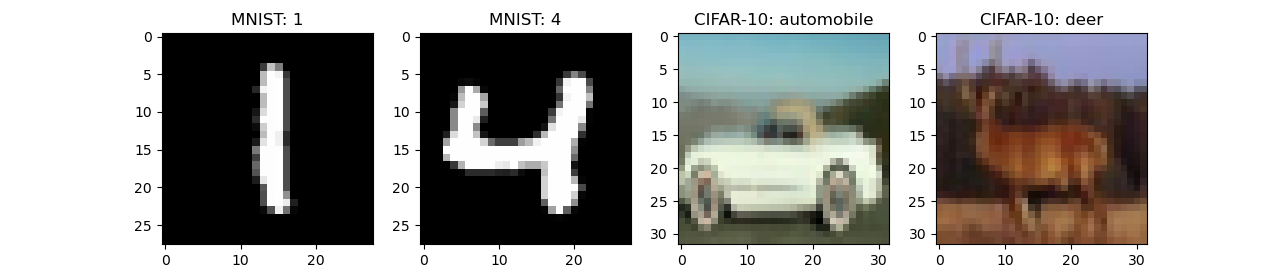
\includegraphics[width=0.45\textwidth]{pictures/dataset.png}
    \caption{数据集预览}
\end{figure}

在本次实验中,对于MNIST数据集和CIFAR-10数据集,我们分别取每类训练集前500张图片为训练集,每类测试集前100张图片为测试集。共计5000张训练图片与1000张测试图片。

\subsubsection{数据预处理}
\paragraph*{归一化}
在实验中,我们对数据进行了归一化处理,将数据的像素值从$[0, 255]$归一化到$[0, 1]$。

通过归一化,我们可以使得数据的特征值在同一量级上,从而加快算法的收敛速度并提高算法的准确率。

\paragraph*{MNIST数据集特征提取}
对于MNIST数据集,我们将$28\times28$的图像展开成一个$784$维的向量,作为SVM的输入特征。

\paragraph*{CIFAR-10数据集特征提取}
对于CIFAR-10数据集,我们通过\verb|skimage|库的\verb|hog()|函数提取图像的梯度直方图(HOG)特征,将图像的$32\times32$的RGB图像转换为$324$维的HOG特征向量,作为SVM的输入特征。

\begin{figure}[H]
    \centering
    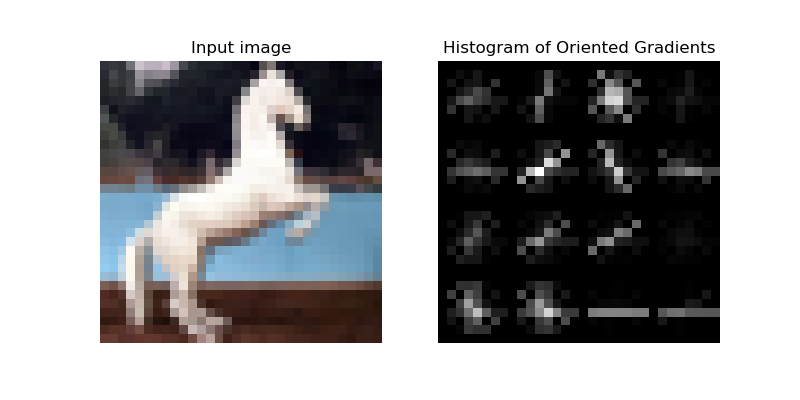
\includegraphics[width=0.45\textwidth]{pictures/hog.png}
    \caption{HOG特征提取}
\end{figure}

\subsubsection{多分类策略}
\paragraph*{OVO策略}
OVO(One-Vs-One)策略是一种多分类策略,即将每两类数据进行一次分类,最终将所有分类结果进行投票,得到最终的分类结果。

\begin{figure}[H]
    \centering
    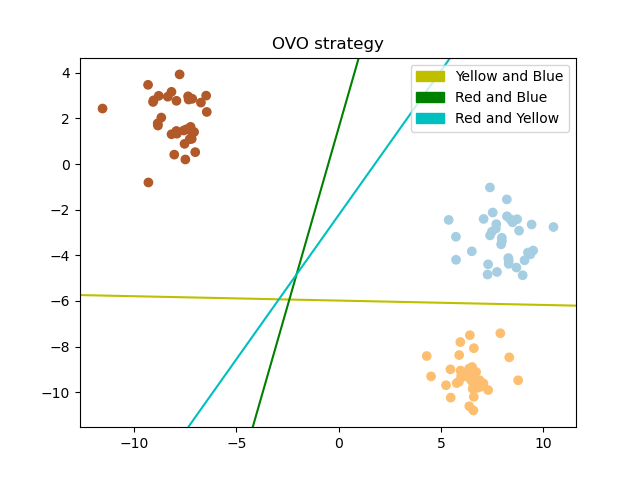
\includegraphics[width=0.45\textwidth]{pictures/OVO.png}
    \caption{OVO策略}
\end{figure}

\paragraph*{OVA策略}
OVA(One-Vs-All)策略是一种多分类策略,即将每一类数据与其他所有类数据进行一次分类,最终将所有分类结果进行投票,得到最终的分类结果。

\begin{figure}[H]
    \centering
    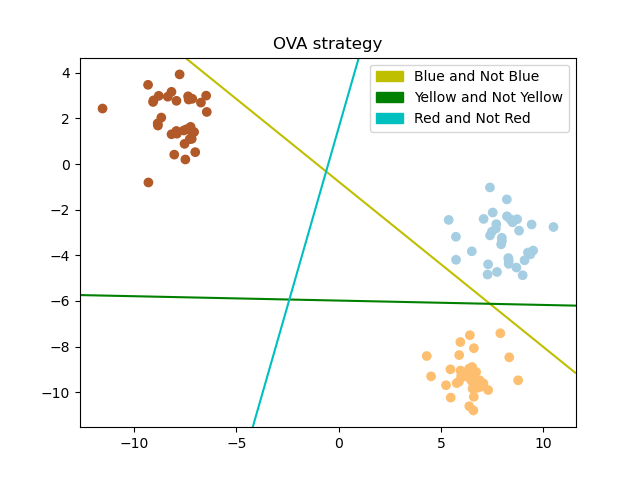
\includegraphics[width=0.45\textwidth]{pictures/OVA.png}
    \caption{OVA策略}
\end{figure}

\paragraph*{策略对比}
在实验中,我们将OVO策略和OVA策略进行对比,分析两种策略的优劣。
通过实验,我们发现OVO策略相较于OVA策略,准确率更高且运行时间更短。

在准确率方面,在OVO策略中,每次训练SVM时,训练数据中两个标签的比例为1:1,而在OVA策略中,训练数据中两个标签的比例为1:9。这导致在OVA策略中出现了类别不平衡,SVM更倾向于将数据分类为数量较多的类别,从而导致准确率下降。

而在运行时间方面,OVO策略中,每次训练SVM时,训练数据量更小,而SMO算法的时间复杂度介于$O(n^2)$和$O(n^3)$之间。OVO策略将数据集分割后训练,每次训练的数据量更小,因此运行时间更短。

\subsection{实验结果}
\subsubsection{单核SVM}
\paragraph*{参数消融}
在实验中,我们对单核SVM算法中的核函数参数进行消融实验,以下是参数消融结果:
\begin{figure}[H]
    \centering
    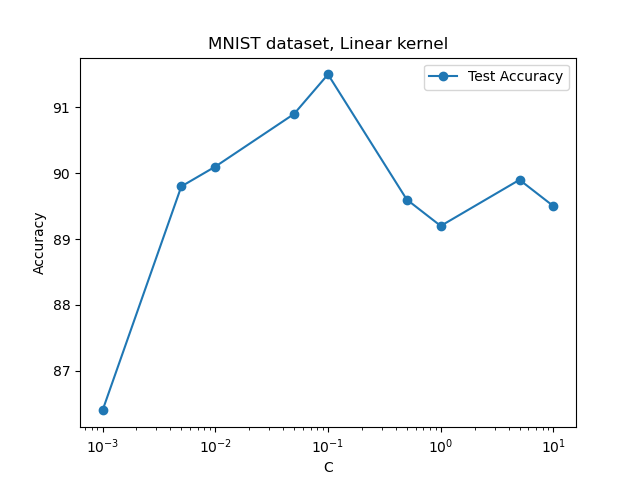
\includegraphics[width=0.35\textwidth]{pictures/single kernel/参数消融+MNIST+线性核.png}
    \caption{MNIST\ +线性核}
\end{figure}
当$C=0.1$时,模型在测试集的准确率最高,为91.1\%。

\begin{figure}[H]
    \centering
    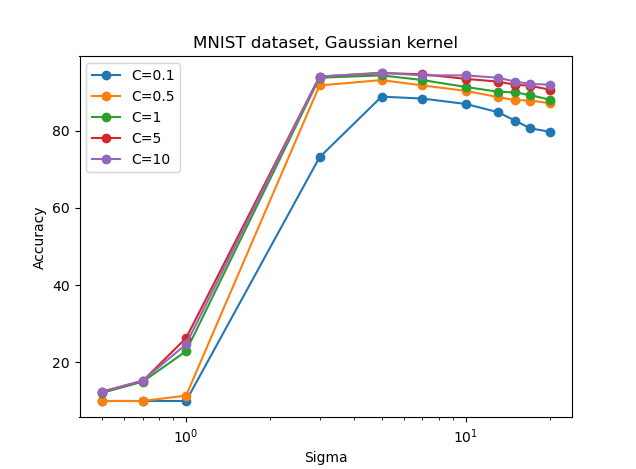
\includegraphics[width=0.35\textwidth]{pictures/single kernel/参数消融+MNIST+高斯核.png}
    \caption{MNIST\ +高斯核}
\end{figure}
当$C=10, \sigma=5$时,模型在测试集的准确率最高,为94.8\%。

\begin{figure}[H]
    \centering
    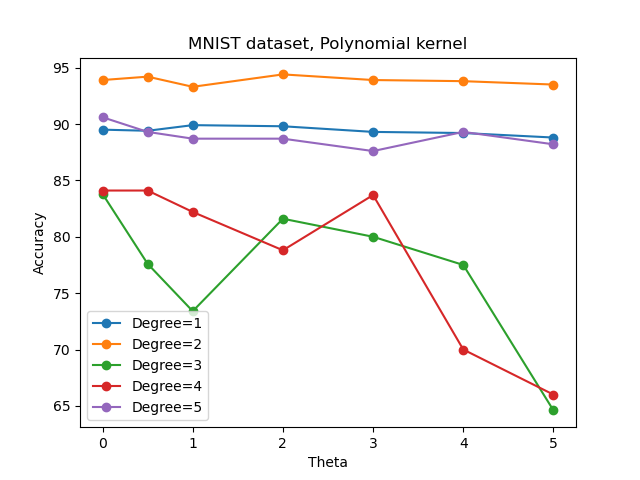
\includegraphics[width=0.35\textwidth]{pictures/single kernel/参数消融+MNIST+多项式核.png}
    \caption{MNIST\ +多项式核}
\end{figure}
当$d=2, \theta=2$时,模型在测试集的准确率最高,为93.7\%。

\begin{figure}[H]
    \centering
    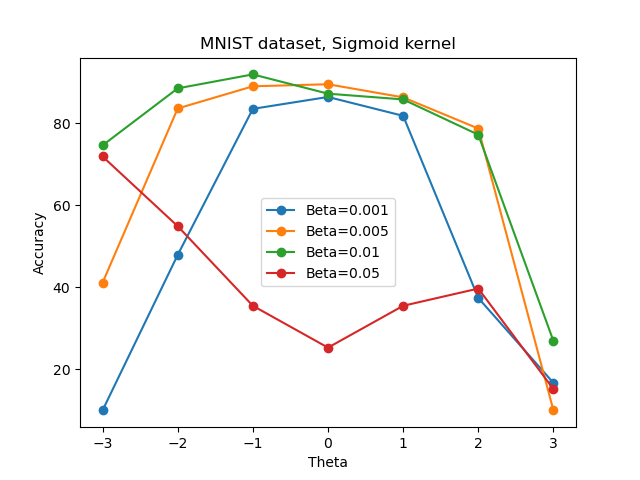
\includegraphics[width=0.35\textwidth]{pictures/single kernel/参数消融+MNIST+sigmoid核.png}
    \caption{MNIST\ +Sigmoid核}
\end{figure}
当$\beta=0.01, \theta=-1$时,模型在测试集的准确率最高,为91.7\%。

\begin{figure}[H]
    \centering
    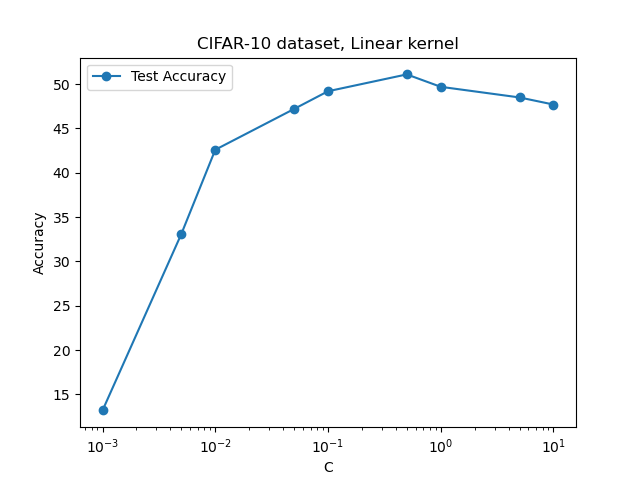
\includegraphics[width=0.35\textwidth]{pictures/single kernel/参数消融+CIFAR10+线性核.png}
    \caption{CIFAR-10\ +线性核}
\end{figure}
当$C=0.5$时,模型在测试集的准确率最高,为50.6\%。

\begin{figure}[H]
    \centering
    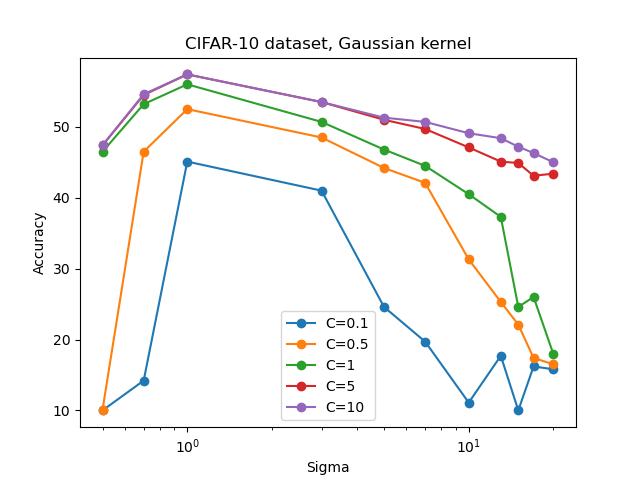
\includegraphics[width=0.35\textwidth]{pictures/single kernel/参数消融+CIFAR10+高斯核.png}
    \caption{CIFAR-10\ +高斯核}
\end{figure}
当$C=10, \sigma=1$时,模型在测试集的准确率最高,为57.4\%。

\begin{figure}[H]
    \centering
    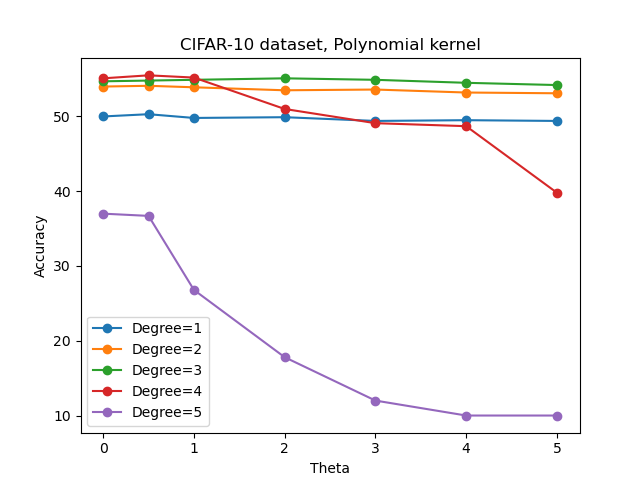
\includegraphics[width=0.35\textwidth]{pictures/single kernel/参数消融+CIFAR10+多项式核.png}
    \caption{CIFAR-10\ +多项式核}
\end{figure}
当$d=4, \theta=0.5$时,模型在测试集的准确率最高,为55.4\%。

\begin{figure}[H]
    \centering
    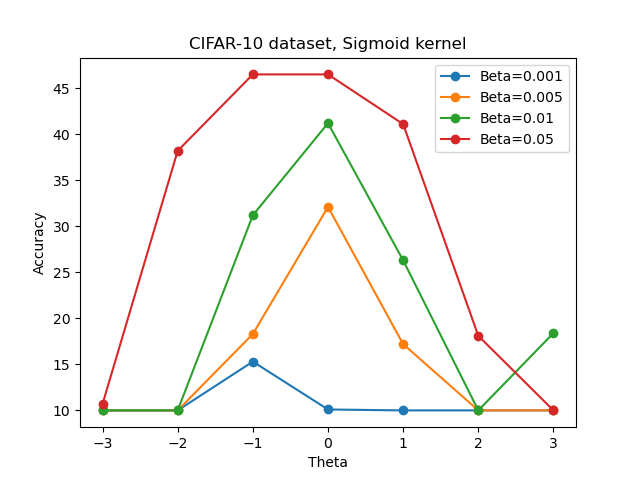
\includegraphics[width=0.35\textwidth]{pictures/single kernel/参数消融+CIFAR10+sigmoid核.png}
    \caption{CIFAR-10\ +Sigmoid核}
\end{figure}
当$\beta=0.05, \theta=-1$时,模型在测试集的准确率最高,46.9\%。


不同核函数在MNIST数据集和CIFAR-10数据集上的最优参数准确率和运行时间见下表:
\begin{table}[H]
  \caption{MNIST数据集}
  \centering
  \begin{tabular}{ c c c c }
    \toprule
    \textbf{核函数} & \textbf{准确率} & \textbf{训练时间} & \textbf{测试时间}\\
    \midrule
    线性核 & 91.1\% & 16.97(s) & 0.70(s) \\
    高斯核 & \textbf{94.8\%} & 179.36(s) & 160.83(s) \\
    多项式核 & 93.7\% & 17.15(s) & 0.85(s) \\
    Sigmoid核 & 91.7\% & 16.74(s) & 1.12(s) \\
    \bottomrule
  \end{tabular}
\end{table}

\begin{table}[H]
  \caption{CIFAR-10数据集}
  \centering
  \begin{tabular}{ c c c c }
    \toprule
    \textbf{核函数} & \textbf{准确率} & \textbf{训练时间} & \textbf{测试时间}\\
    \midrule
    线性核 & 50.6\% & 17.88(s) & 0.59(s) \\
    高斯核 & \textbf{57.4\%} & 96.61(s) & 62.81(s) \\
    多项式核 & 55.4\% & 30.55(s) & 1.31(s) \\
    Sigmoid核 & 46.9\% & 15.81(s) & 0.95(s) \\
    \bottomrule
  \end{tabular}
\end{table}

由上述实验结果可知,对于两个数据集,高斯核函数的效果最好,准确率分别为94.8\%和57.4\%;线性核函数的效率最高,训练时间分别为16.97s和17.88s。

\subsubsection{多核SVM}
\paragraph*{参数消融}
在实验中,我们采用单核SVM中各个核函数的最有参数,对多核SVM算法中的核函数权重进行消融实验,以下是参数消融结果:

\begin{figure}[H]
    \centering
    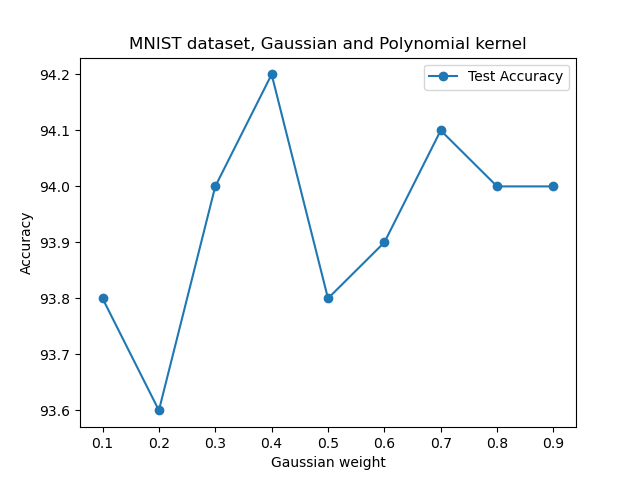
\includegraphics[width=0.35\textwidth]{pictures/multi kernel/MNIST+高斯核+多项式核.png}
    \caption{MNIST\ +高斯核+多项式核}
\end{figure}
当$Gweight=0.4, Pweight=0.6$时,模型在测试集的准确率最高,为94.2\%。

\begin{figure}[H]
    \centering
    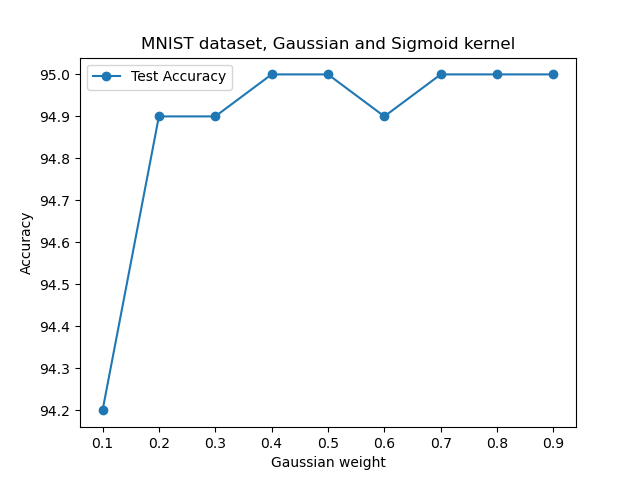
\includegraphics[width=0.35\textwidth]{pictures/multi kernel/MNIST+高斯核+sigmoid核.png}
    \caption{MNIST\ +高斯核+\ Sigmoid核} 
\end{figure}
当$Gweight=0.4/0.5/0.7/0.8/0.9$, \\$Sweight=0.6/0.5/0.3/0.2/0.1$时,模型在测试集的准确率最高,为95.0\%。

\begin{figure}[H]
    \centering
    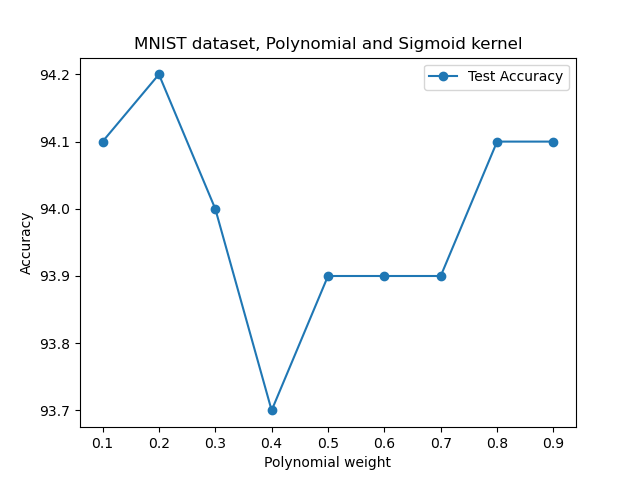
\includegraphics[width=0.35\textwidth]{pictures/multi kernel/MNIST+多项式核+sigmoid核.png}
    \caption{MNIST\ +多项式核+\ Sigmoid核}
\end{figure}
当$Pweight=0.2, Sweight=0.8$时,模型在测试集的准确率最高,为94.2\%。


\begin{figure}[H]
    \centering
    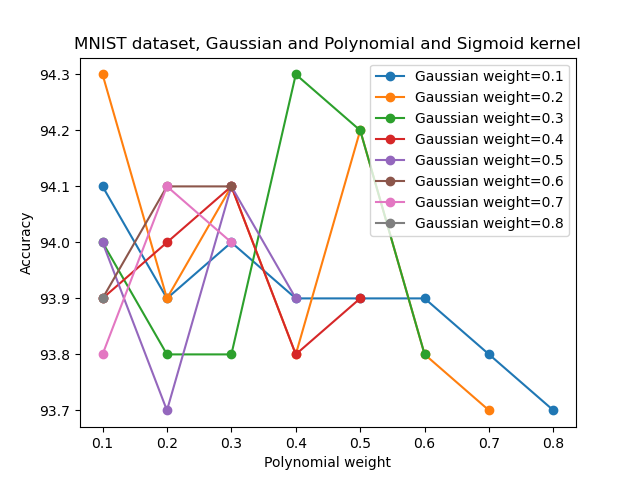
\includegraphics[width=0.35\textwidth]{pictures/multi kernel/MNIST+高斯核+多项式核+sigmoid核.png}
    \caption{MNIST+高斯核+多项式核+Sigmoid核}
\end{figure}
当$Gweight=0.3$, $Pweight=0.4$, \\$Sweight=0.3$时,模型在测试集的准确率最高,为94.3\%。

\begin{figure}[H]
    \centering
    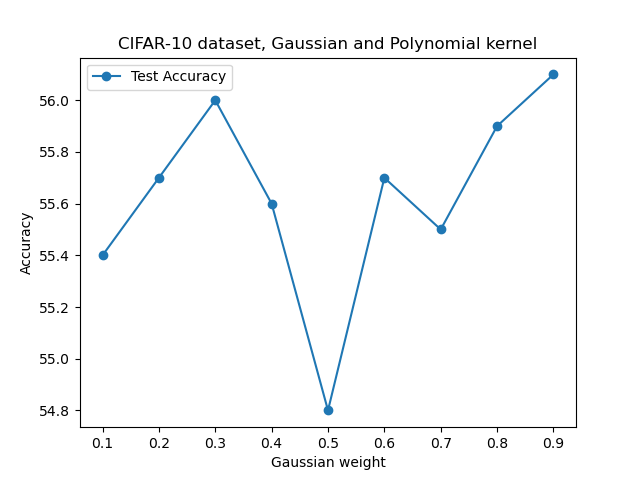
\includegraphics[width=0.35\textwidth]{pictures/multi kernel/CIFAR10+高斯核+多项式核.png}
    \caption{CIFAR-10\ +高斯核+多项式核}
\end{figure}
当$Gweight=0.9, Pweight=0.1$时,模型在测试集的准确率最高,为56.1\%。

\begin{figure}[H]
    \centering
    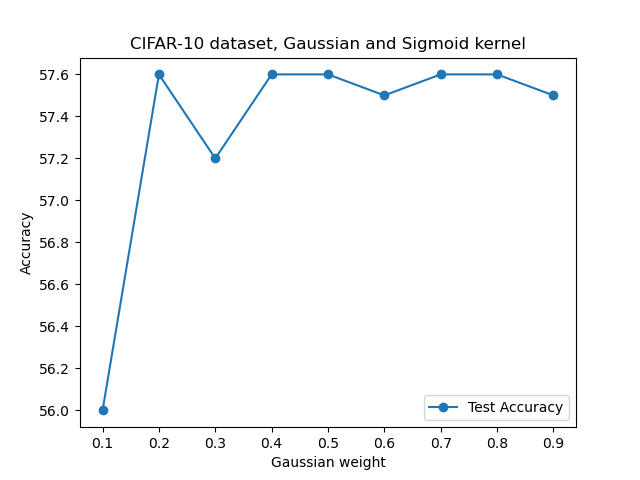
\includegraphics[width=0.35\textwidth]{pictures/multi kernel/CIFAR10+高斯核+sigmoid核.png}
    \caption{CIFAR-10\ +高斯核+\ Sigmoid核}
\end{figure}
当$Gweight=0.2/0.4/0.5/0.7/0.8$, \\$Sweight=0.8/0.6/0.5/0.3/0.2$时,模型在测试集的准确率最高,为57.6\%。

\begin{figure}[H]
    \centering
    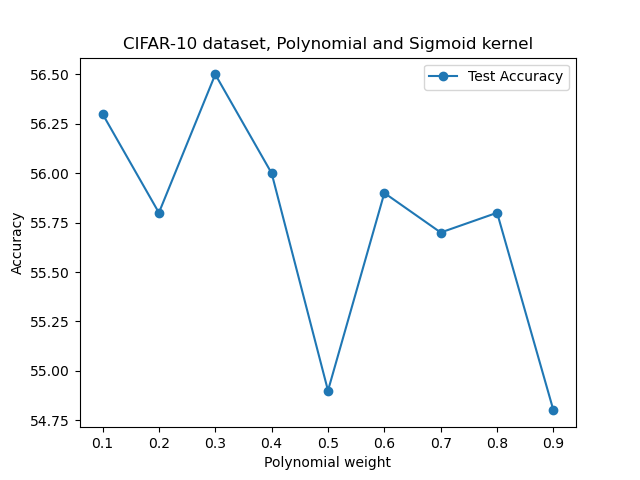
\includegraphics[width=0.35\textwidth]{pictures/multi kernel/CIFAR10+多项式核+sigmoid核.png}
    \caption{CIFAR-10\ +多项式核+\ Sigmoid核}
\end{figure}
当$Pweight=0.3, Sweight=0.7$时,模型在测试集的准确率最高,为56.5\%。

\begin{figure}[H]
    \centering
    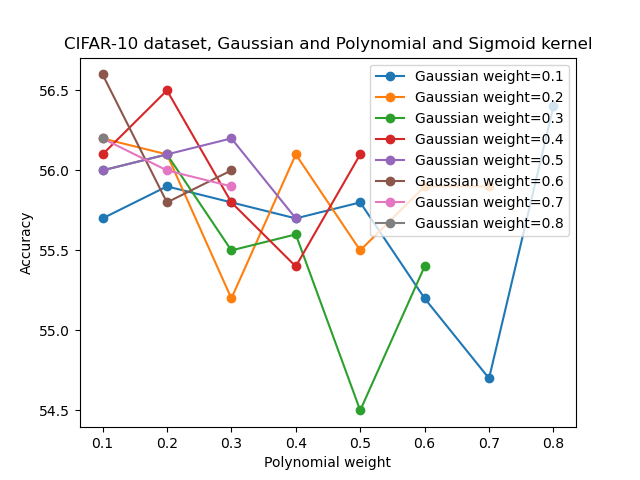
\includegraphics[width=0.35\textwidth]{pictures/multi kernel/CIFAR10+高斯核+多项式核+sigmoid核.png}
    \caption{\fontsize{10}{17}\selectfont CIFAR-10+高斯核+多项式核+sigmoid核}
\end{figure}
当$Gweight=0.6$, $Pweight=0.1$, \\$Sweight=0.3$时,模型在测试集的准确率最高,为56.6\%。

由上述实验结果可知,除了在CIFAR-10上高斯核与Sigmoid核混合之外,当多核SVM的核函数为高斯核与其他核函数混合时,效果都没有单核SVM的高斯核效果好。而高斯核也是单核SVM中效果最好的核函数。由此,我们可以推断,当其他核函数与高斯核混合时,会影响高斯核的效果。

因此,我们尝试将多个参数不同的高斯核混合,核函数参数如下:
\begin{table}[H]
  \caption{高斯核混合}
  \centering
  \begin{tabular}{ c c c }
    \toprule
    \textbf{C} & \textbf{$\sigma$} \\
    \midrule
    9 & 4.5 \\
    10 & 5.0 \\
    11 & 5.5 \\
    \bottomrule
  \end{tabular}
\end{table}

对上述三个高斯核构成的多核函数进行消融实验,以下是参数消融结果:
\begin{figure}[H]
    \centering
    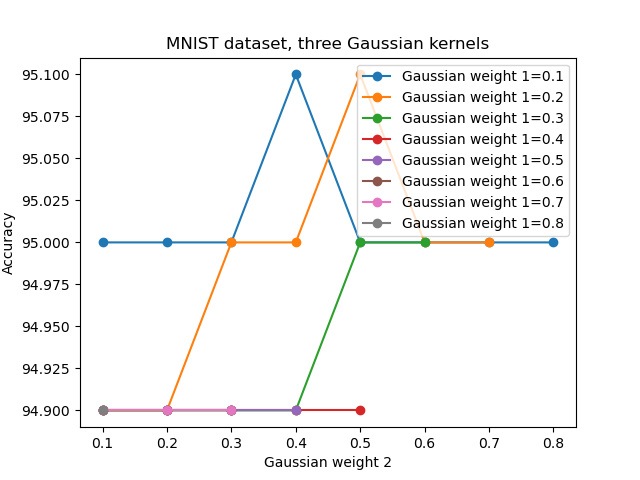
\includegraphics[width=0.35\textwidth]{pictures/multi kernel/MNIST+3高斯核.png}
    \caption{MNIST\ +3个高斯核}
\end{figure}
当$Gweight1=0.1/0.2$, $Gweight2=0.4/0.5$, $Gweight3=0.5/0.3$时,模型在测试集的准确率最高,为95.1\%。

\begin{figure}[H]
    \centering
    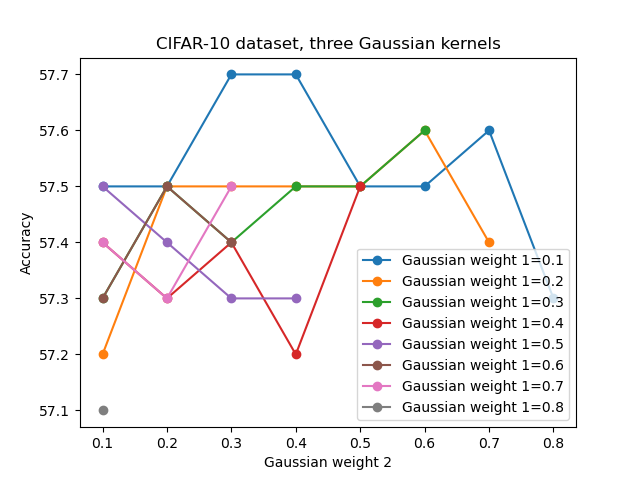
\includegraphics[width=0.35\textwidth]{pictures/multi kernel/CIFAR10+3高斯核.png}
    \caption{CIFAR-10\ +3个高斯核}
\end{figure}
当$Gweight1=0.1$, $Gweight2=0.3/0.4$, $Gweight3=0.6/0.5$时,模型在测试集的准确率最高,为57.7\%。


在MNIST数据集上,模型在测试集的准确率为95.1\%,在CIFAR-10数据集上,模型在测试集的准确率为57.7\%。均略高于单高斯核SVM的效果。

不同多核函数在MNIST数据集和CIFAR-10数据集上的最优参数准确率和运行时间见下表(G:高斯核、P:多项式核、S:Sigmoid核):
\begin{table}[H]
  \caption{MNIST数据集}
  \centering
  \begin{tabular}{ c c c c }
    \toprule
    \textbf{核函数} & \textbf{准确率} & \textbf{训练时间} & \textbf{测试时间} \\
    \midrule
    G+P & 94.2\% & 186.82(s) & 173.95(s) \\
    G+S & 95.0\% & 188.97(s) & 171.34(s) \\
    P+S & 94.2\% & 18.43(s) & 1.83(s) \\
    G+P+S & 94.3\% & 187.91(s) & 172.02(s) \\
    G+G+G & \textbf{95.1\%} & 527.15(s) & 518.82(s) \\
    \bottomrule
  \end{tabular}
\end{table}

\begin{table}[H]
  \caption{CIFAR-10数据集}
  \centering
  \begin{tabular}{ c c c c }
    \toprule
    \textbf{核函数} & \textbf{准确率} & \textbf{训练时间} & \textbf{测试时间}\\
    \midrule
    G+P & 56.1\% & 94.42(s) & 66.22(s) \\
    G+S & 57.6\% & 95.95(s) & 65.83(s) \\
    P+S & 56.5\% & 33.46(s) & 2.61(s) \\
    G+P+S & 56.6\% & 96.94(s) & 67.30(s) \\
    G+G+G & \textbf{57.7\%} & 236.12(s) & 194.98(s) \\
    \bottomrule
  \end{tabular}
\end{table}

\section{总结}
在本次大作业中,我们实现了SVM算法,并在MNIST和CIFAR-10数据集上进行了实验。

在多分类策略上,我们发现OVO策略相较于OVA策略,准确率更高且运行时间更短。并合理分析了这种情况出现的原因。

通过参数消融实验,我们分析了SVM算法中的核函数参数对模型性能的影响。

我们发现,高斯核函数在两个数据集上的效果最好,准确率分别为94.8\%和57.4\%;线性核函数的效率最高,训练时间分别为16.97s和17.88s。

在多核SVM算法中,我们发现高斯核函数与其他核函数混合时,效果不如单核SVM中的高斯核效果好。在尝试将多个参数不同的高斯核混合后,发现效果略高于单高斯核SVM的效果。最终,我们在MNIST数据集上的准确率达到了95.2\%,在CIFAR-10数据集上的准确率达到了57.7\%。 

通过这次大作业,我对SVM算法有了更深入的了解,对SVM算法的核函数、多分类策略等方面有了更深入的认识。同时,我也学会了如何使用Python从零实现SVM算法,并在实际数据集上进行实验。

\section{参考文献}

\begingroup
\renewcommand{\section}[1]{}
\begin{thebibliography}{9}
    \bibitem{smo} 
    Stanford University, CS229 Course. 
    \textit{The Simplified SMO Algorithm}. 
    2009.
\end{thebibliography}
\endgroup

\end{document}
